\documentclass[10pt]{article}
\usepackage[utf8]{inputenc}
\usepackage[T1]{fontenc}
\usepackage{amsmath}
\usepackage{amsfonts}
\usepackage{amssymb}
\usepackage[version=4]{mhchem}
\usepackage{stmaryrd}
\usepackage{graphicx}
\usepackage[export]{adjustbox}
\graphicspath{ {./images/} }

\title{Università di Catania 
 Corso di Laurea in Fisica 
 Compito scritto di Fisica Generale I 
 M.G. Grimaldi - A. Insolia }

\author{}
\date{}


\begin{document}
\maketitle
Per la prova in itinere ( 2 ore) svolgere i problemi: \(3,4,5\)

Catania, 22 Settembre 2022

Per la prova completa (3 ore) svolgere i problemi: \(1,2,3,4\)

\section{Problema n.1}
Un corpo puntiforme di massa \(m=120 \mathrm{~g}\) è a riposo su un piano orizzontale liscio. Dall'istante \(\mathrm{t}=0\) viene sollecitato da una forza di modulo \(F=F_{0}\left[1-e^{-t / \tau}\right]\) con \(F_{0}=27 \mathrm{~N}\) e \(\tau=8 \mathrm{~s}\) e che forma un angolo \(\alpha=35^{\circ}\) con il piano. Determinare:

a) I'stante \(t^{*}\) in cui il corpo abbandona il piano;

b) il lavoro compiuto dalla forza nell'intervallo \(\left[0, t^{*}\right]\).

\section{Problema n.2}
Si consideri una guida sferica di raggio \(\mathrm{R}\) e centro \(O\), posizionata in un piano verticale, sulla quale rotola senza strisciare una palla (sferica) di raggio \(r\) e massa \(m\) (si veda la figura). La palla è inizialmente ferma sulla sommità della guida e, a seguito di una piccola perturbazione, comincia a muoversi verso destra. Sia \(\theta\) l'angolo formato dalla retta che unisce \(O\) con il centro di massa \(G\) della palla, e la direzione verticale (come in figura). Quanto vale \(\theta\) quando la palla si stacca dalla guida?

\begin{center}
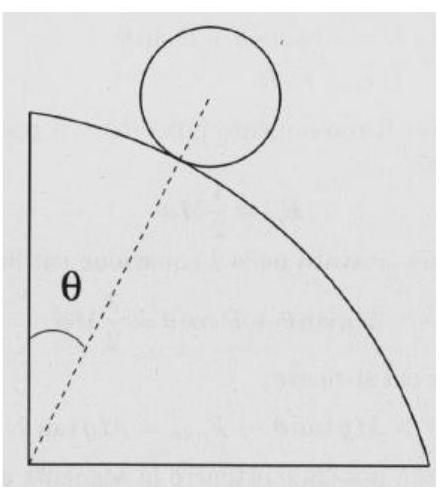
\includegraphics[max width=\textwidth]{2023_05_14_8a9bd4aa7e70f499a317g-1}
\end{center}

\section{Problema n.3}
Una sfera piena di raggio \(\mathrm{R}=10.0 \mathrm{~cm}\) è costituita da un materiale di densità \(\rho\) e viene immersa in acqua (vedi figura).

a) Sapendo che all' equilibrio la linea di galleggiamento della sfera si trova ad una quota \(\mathrm{h}_{0}=4.0 \mathrm{~cm}\) al di sotto del suo vertice superiore (vedi figura) determinare la densità \(\rho\) della sfera.

b) Si supponga, poi, che la sfera, a partire dal suo stato di equilibrio venga spinta leggermente verso il basso e lasciata libera in modo che essa prenda ad oscillare verticalmente. Trascurando la resistenza del mezzo e gli effetti di tensione superficiale, si determini il periodo T delle piccole oscillazioni della sfera intorno alla sua linea di galleggiamento. [Suggerimento 1: per una sfera di raggio \(R\), il volume di una calotta sferica di altezza \(h\) è pari a \(V(h)=(\pi / 3)(3 R-h) h^{2}\). Suggerimento 2: nell'equazione del moto trascurare gli ordini superiori al primo nello spostamento della sfera rispetto alla posizione di equilibrio]

\begin{center}
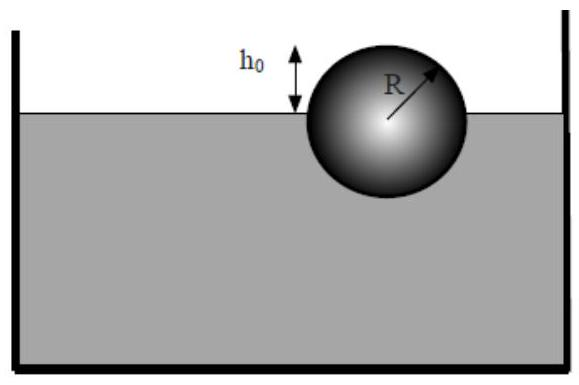
\includegraphics[max width=\textwidth]{2023_05_14_8a9bd4aa7e70f499a317g-2}
\end{center}

\section{Problema n.4}
Un gas ideale monoatomico descrive il ciclo frigorifero in figura. Nello stato \(A\) le variabili termodinamiche del gas sono \(p_{A}=1.20 \times 10^{5} \mathrm{~Pa}, \mathrm{~T}_{\mathrm{A}}=293 \mathrm{~K}, \mathrm{~V}_{\mathrm{A}}=3.0 \times 10^{-3} \mathrm{~m}^{3}\). La trasformazione \(A B\) è una isoterma reversibile, la trasformazione \(B C\) è una adiabatica irreversibile, la trasformazione \(C A\) è una isocora reversibile. Si sa, infine, che \(V_{B}=2 V_{A}, p_{C}=2.00 \times 10^{5} \mathrm{~Pa}\).

a) Calcolare il coefficiente di prestazione del ciclo;

b) Calcolare la variazione di entropia del gas in ogni trasformazione e in un ciclo completo;

c) Calcolare la variazione di entropia dell'universo in un ciclo.

\begin{center}
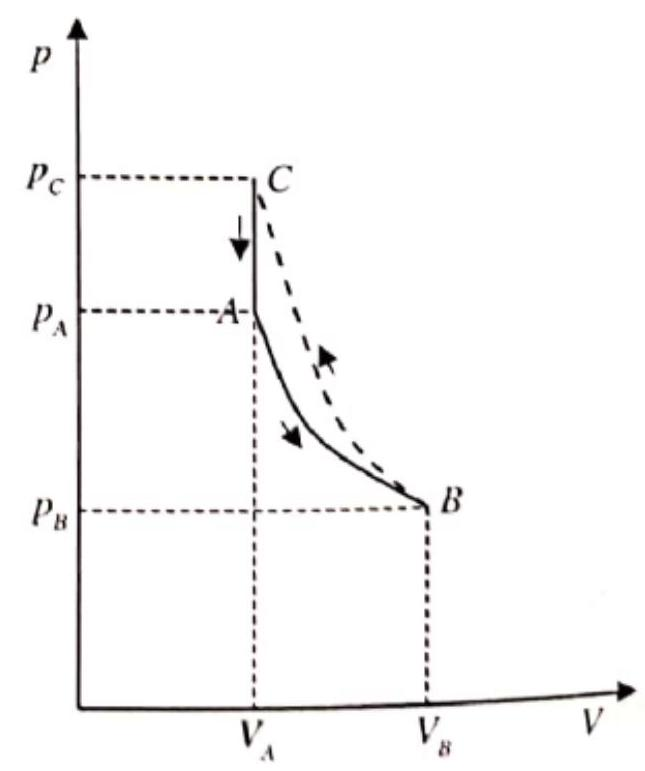
\includegraphics[max width=\textwidth]{2023_05_14_8a9bd4aa7e70f499a317g-2(1)}
\end{center}

\section{Problema n.5}
Si considerino \(n\) moli di idrogeno (gas biatomico, da trattarsi come ideale) che vanno incontro ad una compressione adiabatica reversibile e il cui stato iniziale è caratterizzato da un volume di 10 litri alla temperatura di \(0{ }^{\circ} \mathrm{C}\) e alla pressione di 1 atm e il cui stato finale è caratterizzato da un volume di 1 litro. Si determinino:

a) la variazione di energia interna del gas nella trasformazione;

b) la temperatura del gas nello stato finale;

c) la variazione di entalpia del gas nella trasformazione.


\end{document}